\chapter{System Maintenance}
\section{Environment}
\subsection{Software}
The software that I used to create my system can be found bellow:

\begin{itemize}
\item Python 3
\item IDLE
\item PyQt
\item SQLite 3
\end{itemize}
\subsection{Usage Explanation}
\subsubsection{Python 3}
I used Python 3 mainly because it's the only language that I know well enough to use for a project of this size.
\subsubsection{IDLE}
I used IDLE as it comes with python and it included syntax highlighting specificity for python. I am familiar with this highlighting so it is beneficial for me to use IDLE.
\subsubsection{PyQt}
I used PyQt as it works with python 3 and has integration with SQlite 3 which makes interacting the database much easer.
\subsubsection{SQLite 3}
I used SQLite 3 for my database as it was the only database language that I know, however it has good integration with python 3 and PyQt.
\subsubsection{SQL Inspector}
I used the SQL Inspector as it can help to quickly test and develop SQL code and view any database.

\subsection{Features Used}
\subsubsection{Python 3}
Some of the features that I used include the ability to import from other python files and packages e.g. PyQt.
\subsubsection{IDLE}
I chose to use IDLE as is has specific highlighting for python and I can run the code from IDLE to test it with out, complying it.
\subsubsection{PyQt}
PyQt was used as I found that because Python is an object oriented language it was easy to build the user interface in a way that was easy to understand while programming.
\subsubsection{SQLite 3}
I used SQLite 3 to create a relational database and to search across multiple tables.
\subsubsection{SQL Inspector}
I used the SQL Inspector "Browse Data" function during the development of the CLI interface to identify if my SQL code was working as expected. I also use the "Execute Query" function to help develop more SQL code.

\section{System Overview}


\subsection{System Component}

\section{Code Structure}

%use as many subsections as necessary for the code sections
\subsection{Particular Code Section}
%the code below can be uncommented and used to get a code section from a particular file
\begin{comment}
\begin{figure}[H]
    \pythonfile[firstline=5,lastline=10]{./tex/function_programs/print_function.py}
    \caption{The print() function} \label{fig:print_function}
\end{figure}
\end{comment}

\section{Variable Listing}

\begin{tabular}{|l|l|l|p{4cm}|}
	\hline
	NAME           & DATA TYPE & EXAMPLE DATA & DESCRIPTION                                                       \\ \hline
	current\_table & integer   & 5            & hold the value of the current table as an integer indexing from 0 \\ \hline
	forename & string & Peter & used to hold the forename variable before it is added to the database \\\hline
	surname & string & Millard & used to hold the surname variable before it is added to the database\\\hline
	club &  string & Team Cambridge & used to hold the club name variable before it is added to the database\\\hline
	hold & any & \%bridge\% & used to hold any data temporally be for it is used further in the program \\\hline
	ok & boolean & True & hold the outcome of .prepare function of a SQL query shows if a query was prepared correctly for debugging \\\hline
	data & list & ["peter","Millard",1] & used to hold the SQL query data before it is inserted in to the query \\\hline
	
\end{tabular}

\section{System Evidence}

\subsection{User Interface}

\clearpage

\begin{figure}
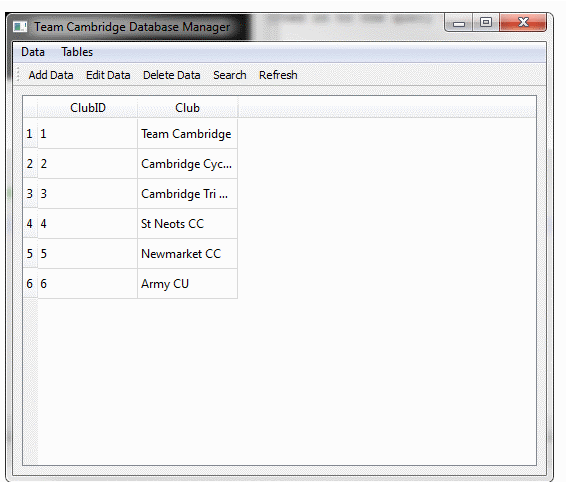
\includegraphics[width=\textwidth]{./Maintenance/UI/Club.png}
\caption{The Club UI} \label{fig:club_UI}
\end{figure}

\begin{figure}
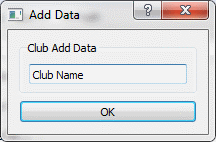
\includegraphics[width=\textwidth]{./Maintenance/UI/ClubAD.png}
\caption{The Club Add Data UI} \label{fig:ClubAD_UI}
\end{figure}

\begin{figure}
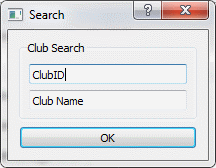
\includegraphics[width=\textwidth]{./Maintenance/UI/ClubSearch.png}
\caption{The Club Search UI} \label{fig:ClubSearch_UI}
\end{figure}

\begin{figure}
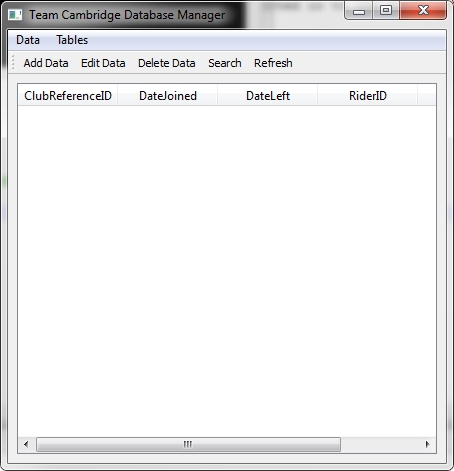
\includegraphics[width=\textwidth]{./Maintenance/UI/ClubRef.png}
\caption{The Club Reference UI} \label{fig:ClubRef_UI}
\end{figure}

\begin{figure}
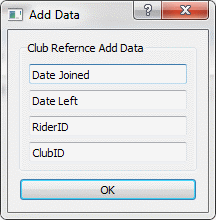
\includegraphics[width=\textwidth]{./Maintenance/UI/ClubRefAD.png}
\caption{The Club Reference Add Data UI} \label{fig:ClubRefAD_UI}
\end{figure}

\begin{figure}
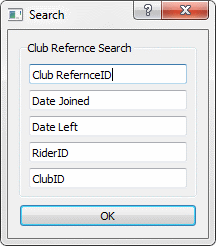
\includegraphics[width=\textwidth]{./Maintenance/UI/ClubRefSearch.png}
\caption{The Club Reference Search UI} \label{fig:ClubRefSearch_UI}
\end{figure}

\begin{figure}
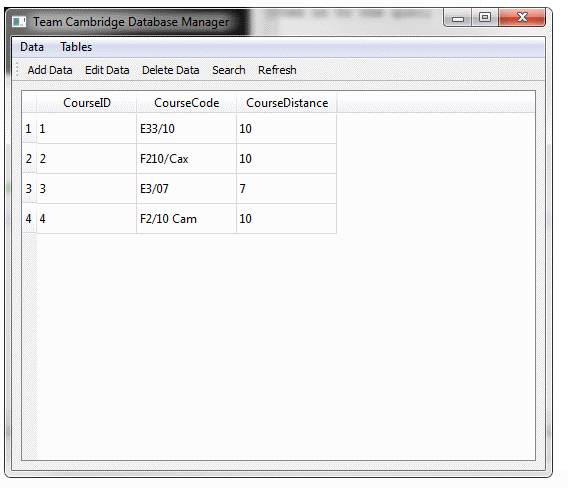
\includegraphics[width=\textwidth]{./Maintenance/UI/Course.png}
\caption{The Course UI} \label{fig:Course_UI}
\end{figure}

\begin{figure}
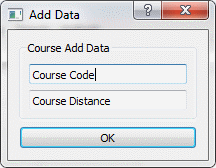
\includegraphics[width=\textwidth]{./Maintenance/UI/CourseAD.png}
\caption{The Course Add Data UI} \label{fig:CourseAD_UI}
\end{figure}

\begin{figure}
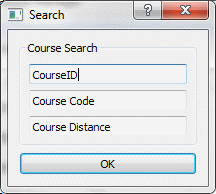
\includegraphics[width=\textwidth]{./Maintenance/UI/CourseSearch.png}
\caption{The Course Search UI} \label{fig:CourseSearch_UI}
\end{figure}

\begin{figure}
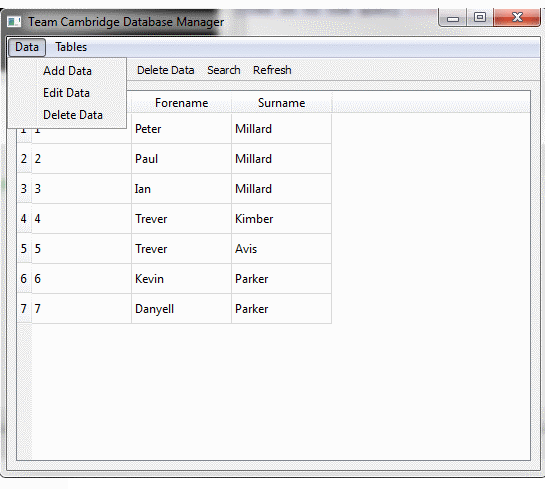
\includegraphics[width=\textwidth]{./Maintenance/UI/DataDrop.png}
\caption{The Data Drop Down Menu UI} \label{fig:DataDrop_UI}
\end{figure}

\begin{figure}
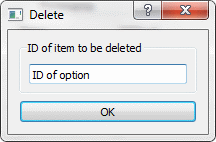
\includegraphics[width=\textwidth]{./Maintenance/UI/Delete.png}
\caption{The Delete UI} \label{fig:Delete_UI}
\end{figure}

\begin{figure}
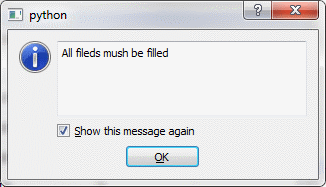
\includegraphics[width=\textwidth]{./Maintenance/UI/Error.png}
\caption{The Error UI} \label{fig:Error_UI}
\end{figure}

\begin{figure}
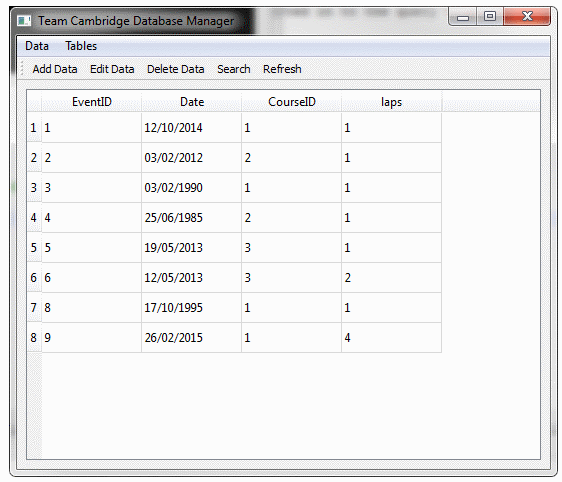
\includegraphics[width=\textwidth]{./Maintenance/UI/Event.png}
\caption{The Event UI} \label{fig:Event_UI}
\end{figure}

\begin{figure}
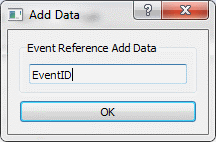
\includegraphics[width=\textwidth]{./Maintenance/UI/EventAD.png}
\caption{The Event Add Data UI} \label{fig:EventAD_UI}
\end{figure}

\begin{figure}
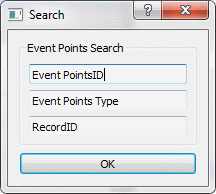
\includegraphics[width=\textwidth]{./Maintenance/UI/EventSearch.png}
\caption{The Event Search UI} \label{fig:EventSearch_UI}
\end{figure}

\begin{figure}
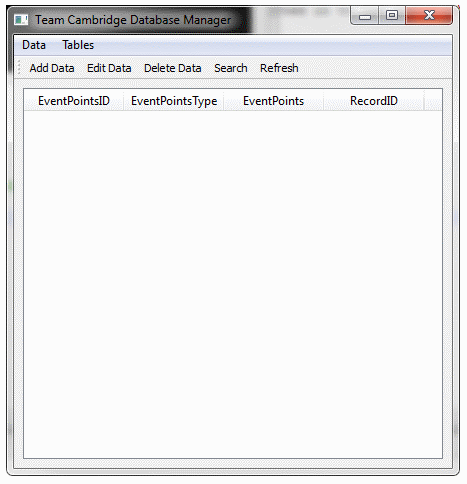
\includegraphics[width=\textwidth]{./Maintenance/UI/EventPoints.png}
\caption{The Event Points UI} \label{fig:EventPoints_UI}
\end{figure}

\begin{figure}
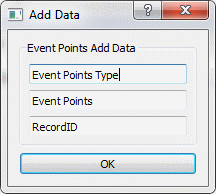
\includegraphics[width=\textwidth]{./Maintenance/UI/EventPointsAD.png}
\caption{The Event Points Add Data UI} \label{fig:EventPointsAD_UI}
\end{figure}

\begin{figure}
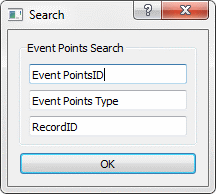
\includegraphics[width=\textwidth]{./Maintenance/UI/EventPointsSearch.png}
\caption{The Event Point Search UI} \label{fig:EventPointsSearch_UI}
\end{figure}

\clearpage

\begin{figure}
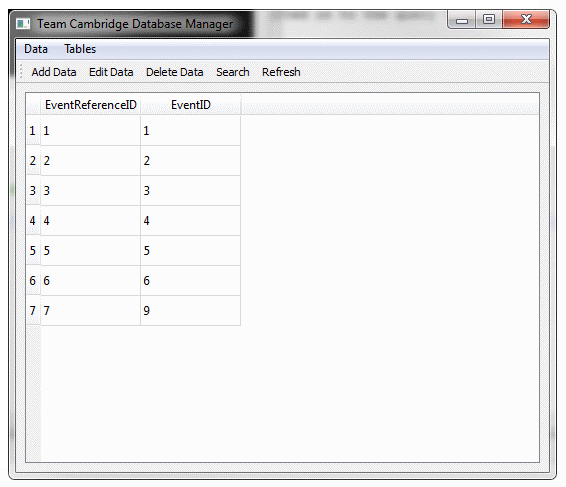
\includegraphics[width=\textwidth]{./Maintenance/UI/EventRef.png}
\caption{The Event Reference UI} \label{fig:EventRef_UI}
\end{figure}

\begin{figure}
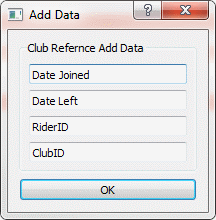
\includegraphics[width=\textwidth]{./Maintenance/UI/EventRefAD.png}
\caption{The Event Reference Add Data UI} \label{fig:EventRefAD_UI}
\end{figure}

\begin{figure}
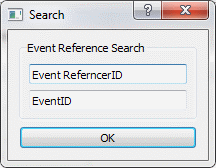
\includegraphics[width=\textwidth]{./Maintenance/UI/EventRefSearch.png}
\caption{The Event Reference Search UI} \label{fig:EventRefSearch_UI}
\end{figure}

\begin{figure}
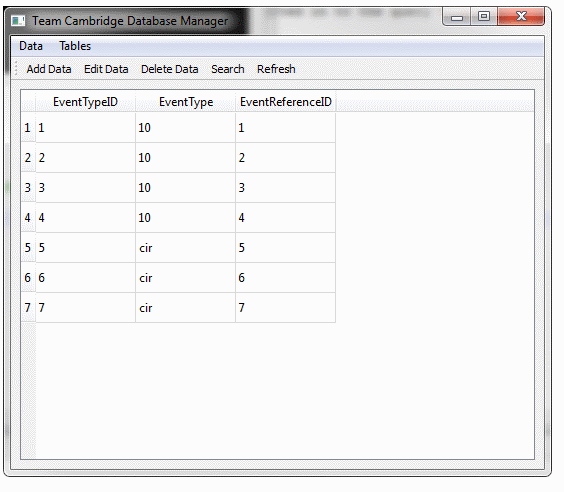
\includegraphics[width=\textwidth]{./Maintenance/UI/EventType.png}
\caption{The Event Type UI} \label{fig:EventType_UI}
\end{figure}

\begin{figure}
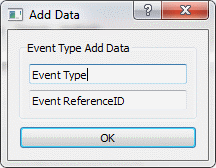
\includegraphics[width=\textwidth]{./Maintenance/UI/EventTypeAD.png}
\caption{The Event Type Add Data UI} \label{fig:EventTypeAD_UI}
\end{figure}

\begin{figure}
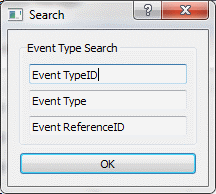
\includegraphics[width=\textwidth]{./Maintenance/UI/EventTypeSearch.png}
\caption{The Event Type Search UI} \label{fig:EventTypeSearch_UI}
\end{figure}

\begin{figure}
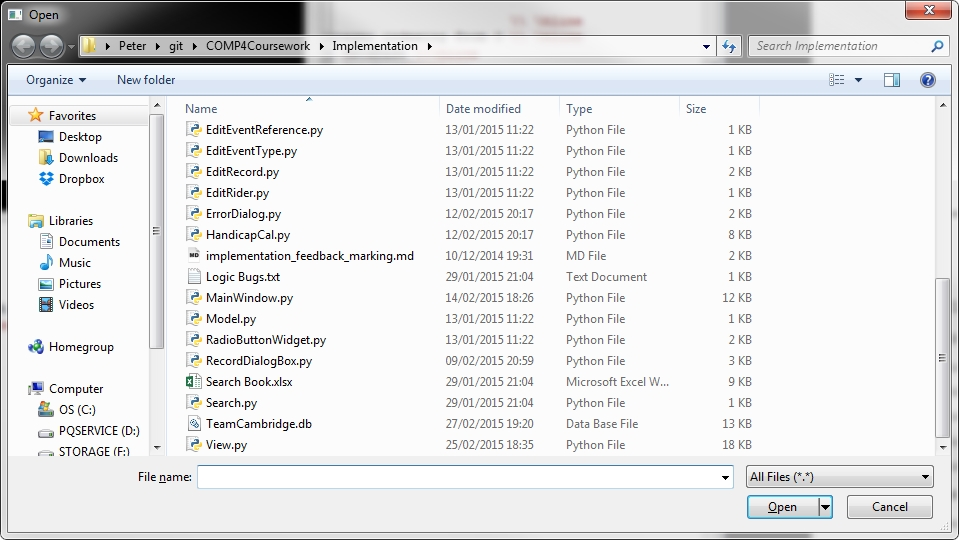
\includegraphics[width=\textwidth]{./Maintenance/UI/FileDia.png}
\caption{The File Dialogue UI} \label{fig:FileDia_UI}
\end{figure}

\begin{figure}
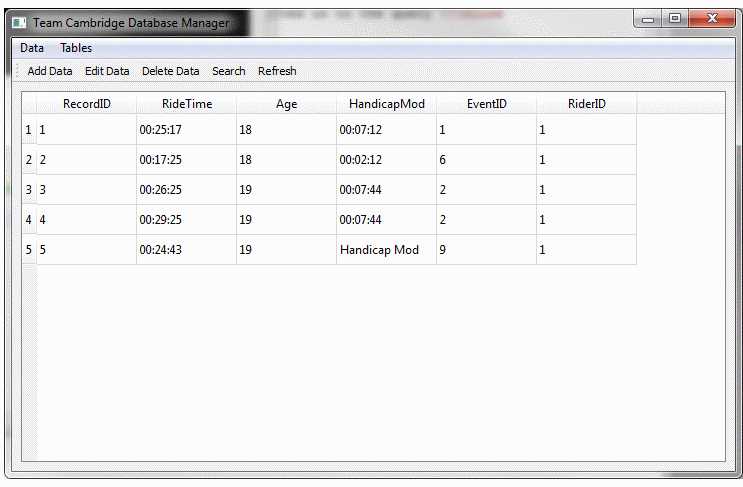
\includegraphics[width=\textwidth]{./Maintenance/UI/Record.png}
\caption{The Record UI} \label{fig:Record_UI}
\end{figure}

\begin{figure}
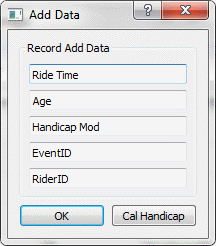
\includegraphics[width=\textwidth]{./Maintenance/UI/RecordAD.png}
\caption{The Record Add Data UI} \label{fig:RecordAD_UI}
\end{figure}

\begin{figure}
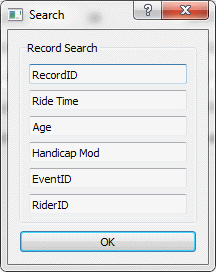
\includegraphics[width=\textwidth]{./Maintenance/UI/RecordSearch.png}
\caption{The Record Search UI} \label{fig:RecordSearch_UI}
\end{figure}

\begin{figure}
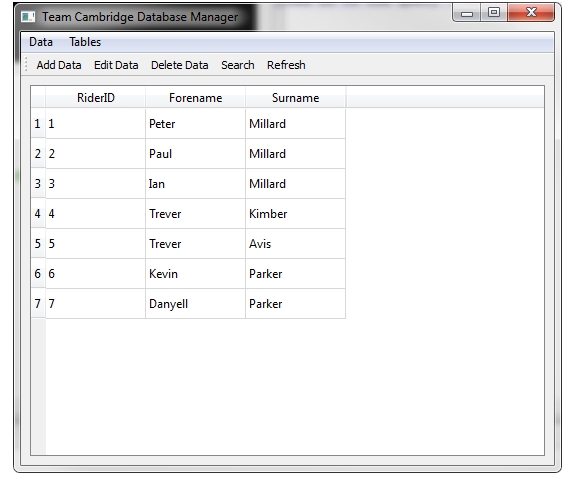
\includegraphics[width=\textwidth]{./Maintenance/UI/Rider.png}
\caption{The Rider UI} \label{fig:Rider_UI}
\end{figure}

\begin{figure}
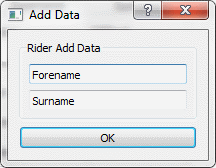
\includegraphics[width=\textwidth]{./Maintenance/UI/RiderAD.png}
\caption{The Rider Add Data UI} \label{fig:RiderAD_UI}
\end{figure}

\begin{figure}
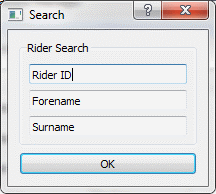
\includegraphics[width=\textwidth]{./Maintenance/UI/RiderSearch.png}
\caption{The Rider Search UI} \label{fig:RdierSearch_UI}
\end{figure}

\begin{figure}
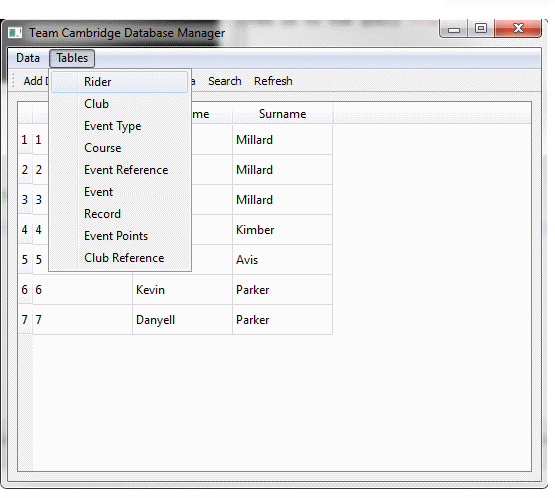
\includegraphics[width=\textwidth]{./Maintenance/UI/TableDrop.png}
\caption{The Table Drop Down UI} \label{fig:TableDrop_UI}
\end{figure}

\clearpage
\subsection{ER Diagram}
\begin{figure}
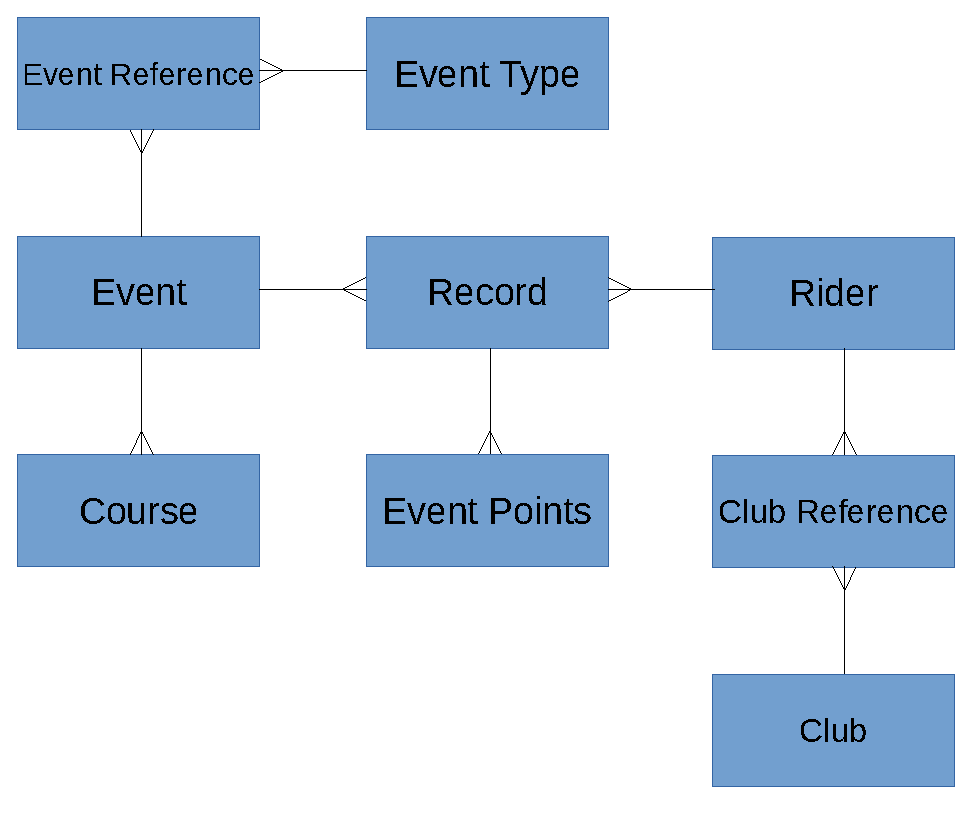
\includegraphics[width=\textwidth]{./Maintenance/ER.pdf}
\caption{The ER Diagram of the final database} \label{fig:ER_Fin}
\end{figure}

\subsection{Database Table Views}
\clearpage

\begin{landscape}
\subsection{Database SQL}
\pythonfile{./Implementation/DatabaseConstructor.py}
\end{landscape}
\subsection{SQL Queries}

SQL code to find the fastest time of a given rider for the handicap calculation of a circuit event:

\pythonfile[firstline=33,lastline=43]{./Implementation/HandicapCal.py}

This querie uses nested querys to find the fasted time of a rider on the E33/10 course, as when calulating the handicap for a circuet event insted for using the fasted time for the same course the fasted time on a E33/10 event is used insted. The primary querie is to find recrods ordered by time, I then used a nested querie to filter the records by EventID and then the EventID is ferther filtered by a second nested querie filtering them by CourseCode. Finaly the resuts are ordered by ride time and the fist in the list should be the fatses time.

SQL code to find the fastest time of a given rider for the handicap calculation of a 10 mile event:

\pythonfile[firstline=52,lastline=62]{./Implementation/HandicapCal.py}

As before I have used nested queries for filtering across mulitpul tables. This querie is used to find the fasted time for a rider on a 10 mile event. 

SQL code to find the fastest time of a given rider for the handicap calculation of a 25 mile event:

\pythonfile[firstline=71,lastline=81]{./Implementation/HandicapCal.py}

\section{Testing}

\subsection{Summary of Results}

\subsection{Known Issues}

\section{Code Explanations}

\subsection{Difficult Sections}

\subsection{Self-created Algorithms}

\section{Settings}
For the system to work as expected you will need to make sure that you have any version of Python 3 and a version of PyQt that is compatible with python 3. All other packages used come with the standard library in python 3.
\section{Acknowledgements}

\section{Code Listing}

\begin{landscape}
\subsection{MianWindow.py}
\pythonfile{./Implementation/MainWindow.py}

\subsection{Connection.py}
\pythonfile{./Implementation/Connection.py}

\subsection{View.py}
\pythonfile{./Implementation/View.py}

\subsection{ErrorDialog.py}
\pythonfile{./Implementation/ErrorDialog.py}

\subsection{CreatingNewRecords.py}
\pythonfile{./Implementation/CreatingNewRecords.py}

\subsection{Search.py}
\pythonfile{./Implementation/Search.py}

\subsection{DialogBox.py}
\pythonfile{./Implementation/DialogBox.py}

\subsection{RecordDialogBox.py}
\pythonfile{./Implementation/RecordDialogBox.py}

\subsection{HandicapCal.py}
\pythonfile{./Implementation/HandicapCal.py}

\subsection{CLI.py}
\pythonfile{./Implementation/CLI.py}

\subsection{Model.py}
\pythonfile{./Implementation/Model.py}

\subsection{DleateData.py}
\pythonfile{./Implementation/DleateData.py}

\subsection{EditClub.py}
\pythonfile{./Implementation/EditClub.py}

\subsection{EditRider.py}
\pythonfile{./Implementation/EditRider.py}

\subsection{EditEventType.py}
\pythonfile{./Implementation/EditEventType.py}

\subsection{EditCourse.py}
\pythonfile{./Implementation/EditCourse.py}

\subsection{EditEventReference.py}
\pythonfile{./Implementation/EditEventReference.py}

\subsection{EditEvent.py}
\pythonfile{./Implementation/EditEvent.py}

\subsection{EditRecord.py}
\pythonfile{./Implementation/EditRecord.py}

\subsection{EditClubReference.py}
\pythonfile{./Implementation/EditClubReference.py}

\subsection{EditEventPoints.py}
\pythonfile{./Implementation/EditEventPoints.py}

\subsection{DatabaseConstructor.py}
\pythonfile{./Implementation/DatabaseConstructor.py}
\end{landscape}
